\begin{figure*}[t]
  \centering
  \begin{tabular}{cccc}
    \hspace{-9mm}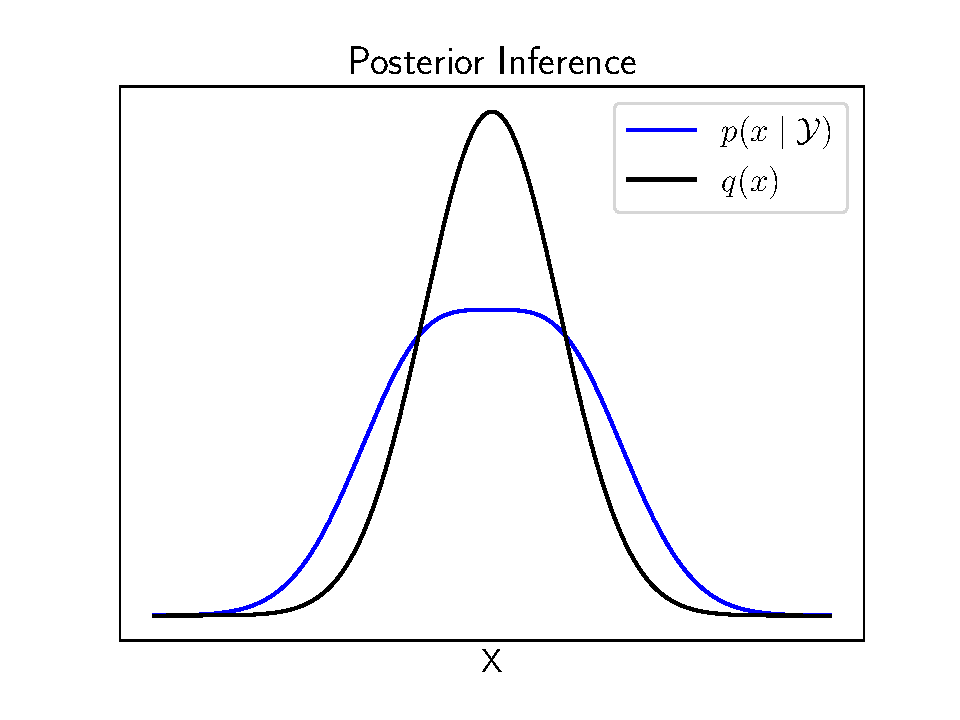
\includegraphics[width=0.29\textwidth]{inf_approx} &
    \hspace{-9mm}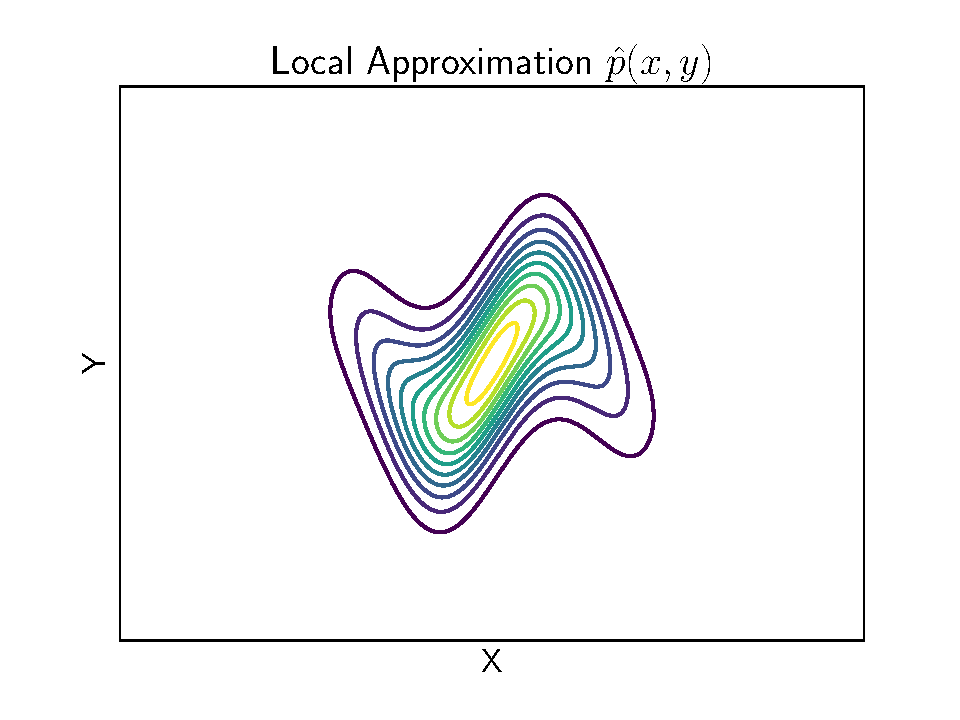
\includegraphics[width=0.29\textwidth]{augmented_dist} &
    \hspace{-9mm}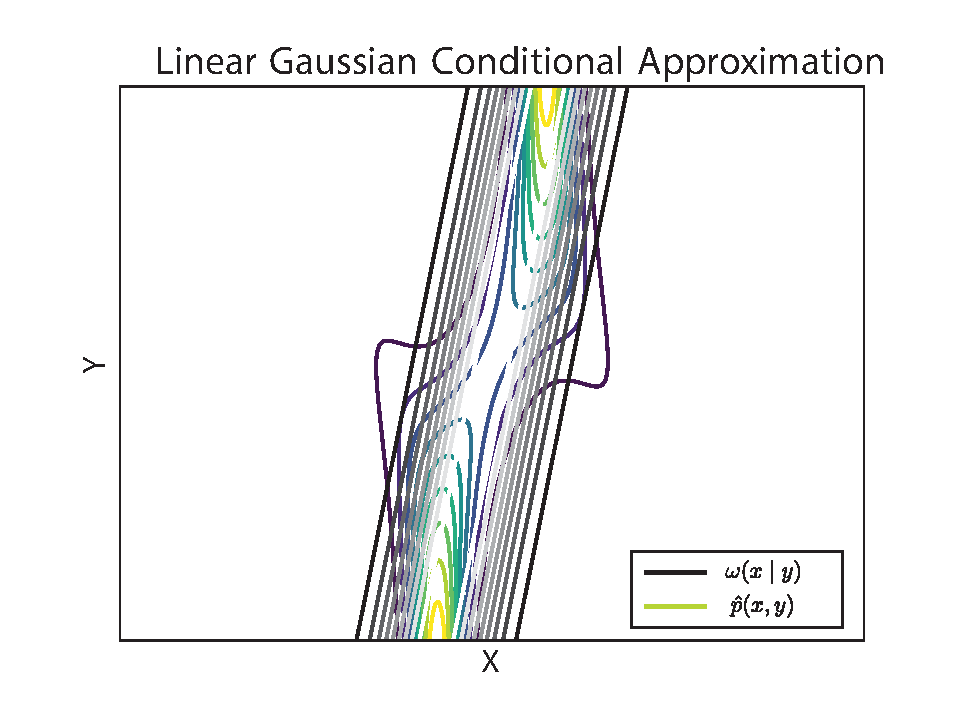
\includegraphics[width=0.29\textwidth]{linear_approx} &
    \hspace{-9mm}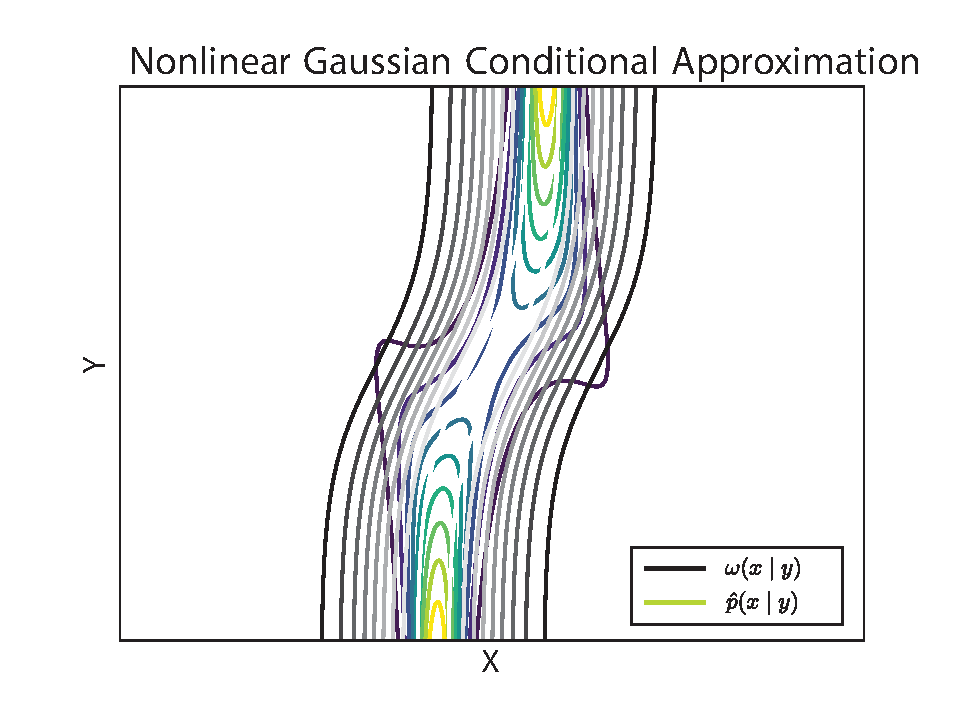
\includegraphics[width=0.29\textwidth]{nonlinear_approx}
  \end{tabular}

  \caption{\small \textbf{Distributional approximations.} \emph{Left:}
  Given observations $\Ycal$ the posterior is approximated with a
  tractable family $q(x) \approx p(x\mid \Ycal)$.  \emph{Center-Left:}
  To consider a new observation $y$, a local approximation is formed
  $\hat{p}(x,y) = q(x) p(y \mid x)$ using the forward model $p(y\mid
  x)$.  \emph{Center-Right:} VIP optimizes a lower bound on MI
  w.r.t.~a distribution $\omega(x\mid y)$ approximating the
  conditional $\hat{p}(x\mid y)$. We use a linear Gaussian
  approximation in this case.  \emph{Right:} Directly parameterizing
  the conditional $\omega(x\mid y)$ allows nonlinear functions of the
  conditioning variable $y$, allowing for better approximations and
  tighter bounds.}

  \label{fig:approx}
\end{figure*}

For any valid distribution $\omega(x\mid y)$, the following is a lower
bound on MI,
\begin{equation}\label{eq:varmi}
  I(X;Y) \geq H(X) + \EE_p[ \log \omega(X\mid Y) ] \equiv \widetilde{I}(X;Y).
\end{equation}
This well-known bound is a result of Gibbs' inequality.  It has been
independently explored for channel coding~\citep{agakov2004algorithm},
reinforcement learning~\citep{mohamed2015variational}, and feature
selection~\citep{gao2016variational, chen2018learning}.
Unfortunately, we cannot directly apply the $\widetilde{I}(X;Y)$
since, in our setting, it involves posterior expectations.

In this section we describe one approach to bounding MI for sequential
planning, which involves a series of approximations.  First, given
past observations $\Ycal$, we approximate the posterior
\mbox{$q(x)\approx p(x\mid \Ycal)$} with a tractable distribution.
Then, a local approximation is formed \mbox{$\hat{p}(x,y) \approx
  p(x,y\mid \Ycal)$} for some future observation $y$.  Finally, we
optimize the auxiliary distribution $\omega(x\mid y)$, which tightens
a lower bound of MI under $\hat{p}(\cdot)$.  See \FIG\ref{fig:approx}
for an illustration.

\subsection{Conditionally Independent Observations}

We begin with the simple model in
\EQN\ref{eq:conditional_indep_joint}, where observations $y$ are
independent conditioned on latent $x$.  Having performed actions
$\Acal_{t-1}$, and observed measurements $\Ycal_{t-1}$, assume that we
have a tractable approximation of the posterior \mbox{$q(x) \approx
  p(x \mid \Ycal_{t-1}, \Acal_{t-1})$}.  We then form a local
approximation of the distribution over a future measurement at time
$t$,
\begin{equation}\label{eq:local_approx}
  \hat{p}_{a}(x,y_t) \equiv q_{t-1}(x) p_{a}(y_t \mid x).
\end{equation}
Here, $p_{a}(y_t \mid x)$ is the true likelihood under the
hypothesized action $a$.  The distribution $\hat{p}(\cdot)$ is
analogous to the \emph{augmented distribution} at each stage of EP
inference, which we will exploit in the next section.  We can then
bound the MI under $\hat{p}(\cdot)$ as,
\begin{equation}\label{eq:varmi_approx}
  H_{\hat{p}}(X) + \max_{a, \,\omega}  \;\EE_{\hat{p}_a}\left[ \log \omega(X \mid Y_{t+1})
  \right].
\end{equation}
We have moved the marginal entropy outside the optimization since it is
constant in this model, and so can be ignored for planning.  The bound
can be evaluated in parallel for a discrete set of actions
$1,\ldots,A$.

\FIG\ref{fig:approx} illustrates the role of each approximation in a
single planning stage, and how the approximations relate to the target
distributions.  To be clear, \EQN\eqref{eq:varmi_approx} bounds mutual
information w.r.t.~the local approximate distribution
$\hat{p}(\cdot)$, not MI under the true posterior.  To ensure that MI
under $\hat{p}(\cdot)$ is a reliable surrogate for posterior MI,
$q(x)$ must accurately approximate the posterior.

\subsection{Annotation Models}

The conditionally independent model of the previous section is a
simple model chosen for illustrative purposes.  We now consider a
different, more complicated distribution, often arising in active
learning~\citep{settles2012active}.  More specifically, consider a
joint distribution over latent $x$, data $\{z_d\}_{d=1}^D$ which are
fixed, and annotations $\{y_d\}_{d=1}^D$,
\[
  p(x,y,z) = p(x) \prod_{d=1}^D p(z_d \mid x) p(y_d \mid z_d). 
\]
For example, $y_d$ may be a discrete class assignment for an image
$z_d$.  

The objective at each learning stage selects the most informative
annotation, \mbox{$\max_d I(X;Y_d \mid \Dcal_{t-1})$}, where
$\Dcal_{t-1}$ represents the set of data and previous annotations
after $t-1$ learning rounds.  MI is computed with respect to the
distribution,
\[
  p(x,y_d \mid \Dcal_{t-1}) \propto p(x \mid \Dcal_{t-1} \setminus \{z_d\}) p(z_d \mid
    x ) p(y_d \mid z_d).
\]
Here, $p(x \mid \Dcal_{t-1} \setminus \{z_d\})$ represents the
posterior distribution after removing $z_d$ from the data.  This step
is algebraic, but intuitively avoids double counting $z_d$.

To form a local approximation we appeal to our connection with the EP
augmented distribution.  We assume an EP-like posterior approximation
which is a product of factor approximations (messages): $q(x) \propto
\prod_{d=1}^D \psi_d(x)$.  The \emph{cavity distribution}
$q^{\backslash d}(x) \propto q(x) / \psi_d(x)$ expresses the posterior
approximation having removed $z_d$.  Our local  approximation is then,
\begin{equation}
  \hat{p}(x, y_d) \propto q^{\backslash d}(x) p(z_d \mid x) p(y_d \mid z_d).
\end{equation}
The MI lower bound is then identical to~\eqref{eq:varmi_approx}.  More
complicated models with nuisance variables that must be integrated out
for planning can be handled in the same manner.  We consider such a
setting for labeled LDA active learning example in
Sec.~\ref{sec:llda}.  
